%%%%%%%%%%%%%%%%%%%%%%%%%%%%%%%%%%%%%%%%%%%%%%%%%%%%%%%%%%%%
% PhonSSM: ICML 2026 Paper
%%%%%%%%%%%%%%%%%%%%%%%%%%%%%%%%%%%%%%%%%%%%%%%%%%%%%%%%%%%%

\documentclass{article}

% Recommended packages
\usepackage{microtype}
\usepackage{graphicx}
\usepackage{subcaption}
\usepackage{caption}
\usepackage{booktabs}

\usepackage{hyperref}
\newcommand{\theHalgorithm}{\arabic{algorithm}}

% For submission (blind review)
\usepackage{icml2026}
% For camera-ready: \usepackage[accepted]{icml2026}

\usepackage{amsmath}
\usepackage{amssymb}
\usepackage{mathtools}
\usepackage{amsthm}
\usepackage{algorithm}
\usepackage{algorithmic}

\usepackage[capitalize,noabbrev]{cleveref}
\usepackage{float}
\usepackage{placeins}
\usepackage{enumitem}
\usepackage[normalem]{ulem}  % For \uline (second-best results)

% Improve float placement
\renewcommand{\topfraction}{0.9}
\renewcommand{\bottomfraction}{0.9}
\renewcommand{\textfraction}{0.1}
\renewcommand{\floatpagefraction}{0.8}

% Theorem environments
\newtheorem{theorem}{Theorem}[section]
\newtheorem{proposition}[theorem]{Proposition}
\newtheorem{lemma}[theorem]{Lemma}
\newtheorem{corollary}[theorem]{Corollary}
\theoremstyle{definition}
\newtheorem{definition}[theorem]{Definition}
\theoremstyle{remark}
\newtheorem{remark}[theorem]{Remark}

% Custom commands
\newcommand{\phonssm}{\textsc{PhonSSM}}
\newcommand{\agan}{\textsc{AGAN}}
\newcommand{\pdm}{\textsc{PDM}}
\newcommand{\bissm}{\textsc{BiSSM}}
\newcommand{\hpc}{\textsc{HPC}}

\icmltitlerunning{State Space Models are Effective Sign Language Learners}

\begin{document}

\twocolumn[
\icmltitle{State Space Models are Effective Sign Language Learners:\\Exploiting Phonological Compositionality for Vocabulary-Scale Recognition}

\icmlsetsymbol{equal}{*}

\begin{icmlauthorlist}
\icmlauthor{Jasper Zhang}{equal,cshl}
\icmlauthor{Bryan Cheng}{equal,cshl}
\end{icmlauthorlist}

\icmlaffiliation{cshl}{Cold Spring Harbor Laboratory, Cold Spring Harbor, NY, USA}

\icmlcorrespondingauthor{Jasper Zhang}{jasperzhang1001@gmail.com}
\icmlcorrespondingauthor{Bryan Cheng}{bcbc7264@gmail.com}

\icmlkeywords{Sign Language Recognition, State Space Models, Graph Neural Networks, Phonological Features, Skeleton-Based Action Recognition}

\vskip 0.3in
]

\printAffiliationsAndNotice{\icmlEqualContribution}

%%%%%%%%%%%%%%%%%%%%%%%%%%%%%%%%%%%%%%%%%%%%%%%%%%%%%%%%%%%%
% ABSTRACT
%%%%%%%%%%%%%%%%%%%%%%%%%%%%%%%%%%%%%%%%%%%%%%%%%%%%%%%%%%%%
\begin{abstract}
Sign language recognition suffers from catastrophic scaling failure: models achieving high accuracy on small vocabularies collapse at realistic sizes. Existing architectures treat signs as atomic visual patterns, learning flat representations that cannot exploit the compositional structure of sign languages---systematically organized from discrete phonological parameters (handshape, location, movement, orientation) reused across the vocabulary. We introduce \phonssm{}, enforcing phonological decomposition through anatomically-grounded graph attention, explicit factorization into orthogonal subspaces, and prototypical classification enabling few-shot transfer. Using skeleton data alone on the largest ASL dataset ever assembled (5,565 signs), \phonssm{} achieves \textbf{72.1\%} on WLASL2000 (+18.4pp over skeleton SOTA), surpassing most RGB methods without video input. Gains are most dramatic in the few-shot regime (+225\% relative), and the model transfers zero-shot to ASL Citizen, exceeding supervised RGB baselines. The vocabulary scaling bottleneck is fundamentally a representation learning problem, solvable through compositional inductive biases mirroring linguistic structure.
\end{abstract}

%%%%%%%%%%%%%%%%%%%%%%%%%%%%%%%%%%%%%%%%%%%%%%%%%%%%%%%%%%%%
% INTRODUCTION
%%%%%%%%%%%%%%%%%%%%%%%%%%%%%%%%%%%%%%%%%%%%%%%%%%%%%%%%%%%%
\section{Introduction}

Sign language recognition systems must distinguish thousands of signs differing in subtle hand configurations, spatial locations, and temporal dynamics---a challenging perceptual problem that current approaches treat as generic sequence classification. Standard architectures (LSTMs \citep{hochreiter1997lstm}, Transformers \citep{vaswani2017attention}, GCNs \citep{kipf2017semi}) learn implicit representations without leveraging the rich linguistic structure that makes sign languages learnable by humans.

\textbf{The phonological insight.} Sign languages, like spoken languages, have phonological structure. Just as spoken words decompose into phonemes, signs decompose into \textit{cheremes}---minimal contrastive units including handshape, location, movement, and orientation \citep{stokoe1960sign, battison1978lexical}. The sign for ``mother'' differs from ``father'' only in location (chin vs.\ forehead); ``chair'' differs from ``sit'' primarily in movement. This compositional structure reflects how signers perceive and produce signs, and how children acquire sign language.

\textbf{Why current approaches fall short.} Standard neural architectures provide no guarantees about what features they capture. A Transformer may distinguish ``mother'' from ``father,'' but nothing ensures it has learned the location contrast that generalizes to other minimal pairs. This leads to poor few-shot performance: models struggle with novel signs even when they share phonological components with training examples. The lack of interpretability hinders error analysis and targeted improvement.

\begin{figure*}[!t]
\centering
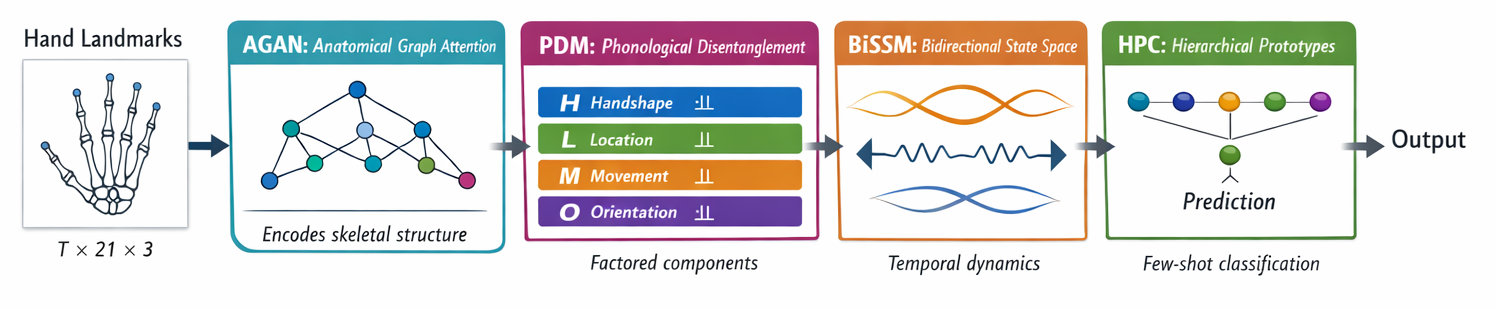
\includegraphics[width=\textwidth]{figures/fig_architecture_final.png}
\vspace{-3mm}
\caption{\textbf{PhonSSM architecture.} Hand landmarks ($T \times 21 \times 3$) flow through four stages: (1)~\agan{} encodes skeletal structure via anatomically-informed graph attention; (2)~\pdm{} factorizes features into four orthogonal phonological components (handshape, location, movement, orientation); (3)~\bissm{} models bidirectional temporal dynamics; (4)~\hpc{} classifies using hierarchical prototypes for few-shot generalization. Total: 3.2M parameters.}
\label{fig:architecture}
\vspace{-2mm}
\end{figure*}

\textbf{Our approach.} We introduce \phonssm{}, an architecture that makes phonological structure explicit. Rather than hoping the model discovers relevant features, we build in the decomposition: separate pathways for handshape, location, movement, and orientation, with explicit factorization objectives. The model learns to recognize signs by composing phonological components, mirroring how linguists and signers conceptualize sign structure.

The architecture has four stages (Figure~\ref{fig:architecture}):
\begin{enumerate}[nosep,topsep=2pt]
\item \textbf{Anatomical Graph Attention Network (\agan{})}: Encodes hand landmarks using graph attention with anatomically-informed connectivity, capturing the kinematic constraints of hand articulation.
\item \textbf{Phonological Disentanglement Module (\pdm{})}: Decomposes spatial features into four phonological subspaces with orthogonality regularization to encourage decorrelated representations.
\item \textbf{Bidirectional Selective State Space (\bissm{})}: Models temporal dynamics using state space models, capturing both forward and backward context efficiently.
\item \textbf{Hierarchical Prototypical Classifier (\hpc{})}: Classifies signs using learned prototypes at both component and sign levels, enabling few-shot generalization.
\end{enumerate}%

\textbf{Why skeleton-based recognition?} We focus on pose/skeleton input extracted via MediaPipe, rather than raw video. This choice offers three advantages: (1) \textit{privacy preservation}---no facial appearance or background information is needed; (2) \textit{computational efficiency}---processing 63-225 landmark coordinates per frame is orders of magnitude cheaper than video; (3) \textit{domain invariance}---skeleton representations abstract away lighting, clothing, and camera variations.

\textbf{Contributions.} This work advances skeleton-based sign language recognition in four ways: (i)~we formalize \emph{phonology as inductive bias}, with explicit handshape, location, movement, and orientation pathways and orthogonality-regularized factorization---to our knowledge, the first architecture to embed phonological structure directly into the model design; (ii)~we integrate anatomical graph attention, phonological decomposition, bidirectional state space modeling, and hierarchical prototypical classification into a unified 3.2M-parameter architecture; (iii)~we construct \emph{Merged-5565}, a new large-scale ASL benchmark combining six sources with 5,565 signs and 260K samples---the largest publicly available isolated sign dataset; and (iv)~we achieve state-of-the-art results with substantial margins: 88.4\% on WLASL100 (+14pp over prior skeleton methods), \textbf{72.1\% on WLASL2000} (+18.4pp over DSTA-SLR), and 53.3\% on Merged-5565 (+26pp over Bi-LSTM), with interpretable phonological confusions.

%%%%%%%%%%%%%%%%%%%%%%%%%%%%%%%%%%%%%%%%%%%%%%%%%%%%%%%%%%%%
% BACKGROUND
%%%%%%%%%%%%%%%%%%%%%%%%%%%%%%%%%%%%%%%%%%%%%%%%%%%%%%%%%%%%
\section{Background: Sign Language Phonology}
\label{sec:background}

Understanding why phonological structure matters requires brief background on sign language linguistics.

\subsection{Phonological Parameters}

Since Stokoe's foundational work \citep{stokoe1960sign}, linguists have analyzed signs as compositions of simultaneous parameters:

\begin{itemize}[nosep,topsep=2pt]
\item \textbf{Handshape}: The configuration of fingers---fist, flat hand, pointing index, etc. ASL uses approximately 30 distinct handshapes \citep{battison1978lexical}.
\item \textbf{Location}: Where the sign is produced---forehead, chin, chest, neutral space. Approximately 15 major locations are distinguished.
\item \textbf{Movement}: The trajectory of the hand(s)---linear, circular, repeated, etc. Movement is often the most salient temporal feature.
\item \textbf{Orientation}: The direction the palm faces---toward signer, away, up, down. Eight orientations are typically distinguished.
\end{itemize}%

Signs that differ in only one parameter form \textit{minimal pairs}, analogous to ``bat'' vs. ``pat'' in English. This structure is not arbitrary: it reflects constraints on human perception and production, and it underlies how sign languages are acquired and processed.

Phonological decomposition provides computational advantages: (1)~\textit{compositionality}---a vocabulary of 5,000 signs can be represented as combinations of $\sim$63 phonological units; (2)~\textit{generalization}---novel signs sharing components with known signs can be recognized more easily; (3)~\textit{interpretability}---phonological features provide vocabulary for describing model behavior.

\subsection{Problem Formulation}

Given a sequence of hand landmarks $\mathbf{X} = (\mathbf{x}_1, \ldots, \mathbf{x}_T)$ where $\mathbf{x}_t \in \mathbb{R}^{N \times C}$ represents $N$ landmarks with $C$ coordinates at time $t$, we aim to predict the sign class $y \in \{1, \ldots, K\}$. The key insight is that this mapping should factor through phonological representations:
\begin{equation}
\mathbf{X} \xrightarrow{\text{spatial}} \mathbf{Z} \xrightarrow{\text{phon.}} (\mathbf{h}, \mathbf{l}, \mathbf{m}, \mathbf{o}) \xrightarrow{\text{temporal}} \mathbf{F} \xrightarrow{\text{classify}} y
\end{equation}
where $\mathbf{h}, \mathbf{l}, \mathbf{m}, \mathbf{o}$ are handshape, location, movement, and orientation representations respectively.

%%%%%%%%%%%%%%%%%%%%%%%%%%%%%%%%%%%%%%%%%%%%%%%%%%%%%%%%%%%%
% METHOD
%%%%%%%%%%%%%%%%%%%%%%%%%%%%%%%%%%%%%%%%%%%%%%%%%%%%%%%%%%%%
\section{Method}
\label{sec:method}

\textbf{Notation.} Let $\mathbf{X} \in \mathbb{R}^{T \times N \times C}$ denote input landmarks with $T$ frames, $N=21$ hand landmarks, and $C=3$ coordinates. We use $D$ for model dimension, $D_c$ for component dimension, and $D_s$ for SSM state dimension.

\subsection{Anatomical Graph Attention Network (AGAN)}

Hand landmarks form a graph $\mathcal{G} = (\mathcal{V}, \mathcal{E})$ with $|\mathcal{V}| = N$ nodes.

\textbf{Graph construction.} The adjacency matrix $\mathbf{A} \in \{0,1\}^{N \times N}$ encodes skeletal connectivity: finger chains (wrist$\to$MCP$\to$PIP$\to$DIP$\to$tip), palm connections, and functional finger pairs.

\textbf{Graph attention layer.} For each frame $t$, let $\mathbf{H}_t^{(0)} = \mathbf{W}_{\text{in}} \mathbf{X}_t \in \mathbb{R}^{N \times D'}$ where $\mathbf{W}_{\text{in}} \in \mathbb{R}^{D' \times C}$. At layer $l$, for head $k \in \{1,\ldots,K\}$:
\begin{equation}
e_{ij}^{(l,k)} = \text{LeakyReLU}\left(\mathbf{a}^{(k)T} [\mathbf{W}^{(l,k)} \mathbf{h}_i^{(l)} \| \mathbf{W}^{(l,k)} \mathbf{h}_j^{(l)}]\right)
\end{equation}
where $\mathbf{W}^{(l,k)} \in \mathbb{R}^{(D'/K) \times D'}$, $\mathbf{a}^{(k)} \in \mathbb{R}^{2D'/K}$, and $\|$ denotes concatenation. Attention weights are normalized over anatomical neighbors:
\begin{equation}
\alpha_{ij}^{(l,k)} = \frac{\exp(e_{ij}^{(l,k)}) \cdot A_{ij}}{\sum_{j' \in \mathcal{N}(i)} \exp(e_{ij'}^{(l,k)}) \cdot A_{ij'}}
\end{equation}
where $\sum_{j} \alpha_{ij}^{(l,k)} = 1$ for all $i, k$. Multi-head aggregation:
\begin{equation}
\mathbf{h}_i^{(l+1)} = \sigma\left( \Big\|_{k=1}^{K} \sum_{j \in \mathcal{N}(i)} \alpha_{ij}^{(l,k)} \mathbf{W}^{(l,k)} \mathbf{h}_j^{(l)} \right)
\end{equation}
After $L$ layers, we mean-pool over nodes: $\mathbf{z}_t = \frac{1}{N} \sum_{i=1}^{N} \mathbf{h}_{t,i}^{(L)} \in \mathbb{R}^{D}$.

\subsection{Phonological Factorization Module (PDM)}

The \pdm{} factorizes spatial features into four component subspaces via parallel MLPs. We use ``factorization'' rather than ``disentanglement'' to clarify this is architectural separation with soft orthogonality constraints, not statistical independence.

\textbf{Component encoders.} Four parallel 2-layer MLPs with shared input:
\begin{equation}
\mathbf{c}_t^{(i)} = \text{MLP}_i(\mathbf{z}_t) \in \mathbb{R}^{D_c}, \quad i \in \{\text{hand}, \text{loc}, \text{mov}, \text{ori}\}
\end{equation}
where $\text{MLP}_i: \mathbb{R}^D \to \mathbb{R}^{D_c}$ with LayerNorm \citep{ba2016layer} and dropout.

\textbf{Movement temporal convolution.} Movement is temporally extended:
\begin{equation}
\tilde{\mathbf{c}}_t^{(\text{mov})} = \mathbf{c}_t^{(\text{mov})} + \text{Conv1D}_{k=5}(\mathbf{C}^{(\text{mov})})_t
\end{equation}
where $\mathbf{C}^{(\text{mov})} \in \mathbb{R}^{T \times D_c}$ and $\text{Conv1D}_{k=5}$ has kernel size 5.

\textbf{Fused representation.} Components are concatenated and projected:
\begin{equation}
\mathbf{f}_t = \mathbf{W}_{\text{fuse}} [\mathbf{c}_t^{(\text{hand})} \| \mathbf{c}_t^{(\text{loc})} \| \tilde{\mathbf{c}}_t^{(\text{mov})} \| \mathbf{c}_t^{(\text{ori})}] \in \mathbb{R}^{D}
\end{equation}
where $\mathbf{W}_{\text{fuse}} \in \mathbb{R}^{D \times 4D_c}$.

\textbf{Orthogonality loss.} We encourage decorrelation at both sequence and frame levels:
\begin{equation}
\mathcal{L}_{\text{ortho}} = \underbrace{\sum_{i \neq j} \cos^2(\bar{\mathbf{c}}^{(i)}, \bar{\mathbf{c}}^{(j)})}_{\text{sequence-level}} + \frac{\lambda_f}{T} \underbrace{\sum_{t=1}^{T} \sum_{i \neq j} \cos^2(\mathbf{c}_t^{(i)}, \mathbf{c}_t^{(j)})}_{\text{frame-level}}
\end{equation}
where $\bar{\mathbf{c}}^{(i)} = \frac{1}{T}\sum_t \mathbf{c}_t^{(i)}$ and $\lambda_f = 0.1$. This addresses temporal structure concerns.

\subsection{Bidirectional Selective State Space (BiSSM)}

We adapt the selective SSM formulation from Mamba \citep{gu2023mamba} for bidirectional temporal modeling. Unlike Transformers with $O(T^2)$ attention, SSMs process sequences in $O(T)$ time while maintaining long-range dependencies through learned state dynamics.

\textbf{Core mechanism.} The SSM maintains a hidden state $\mathbf{x}_t \in \mathbb{R}^{D_s}$ that summarizes temporal context. State transitions and outputs are governed by input-dependent parameters $(\mathbf{A}, \mathbf{B}_t, \mathbf{C}_t, \Delta_t)$, allowing selective emphasis on relevant timesteps. The discretization step $\Delta_t$ controls how much each input updates the state---critical for variable-rate sign movements.

\textbf{Bidirectional processing.} Signs require both anticipatory and retrospective context (e.g., movement direction is only clear after seeing the trajectory). We run forward and backward SSMs in parallel and combine:
\begin{equation}
\mathbf{g}_t = \mathbf{W}_{\text{out}}[\text{SSM}_\rightarrow(\mathbf{F})_t \| \text{SSM}_\leftarrow(\mathbf{F})_t] \in \mathbb{R}^D
\end{equation}
We stack $L_{\text{ssm}}=4$ layers with residual connections. Full parameterization details are in Appendix~\ref{app:bissm}.

\subsection{Hierarchical Prototypical Classifier (HPC)}

\textbf{Component prototypes.} Learnable prototype banks:
\begin{equation}
\mathbf{P}^{(i)} \in \mathbb{R}^{N_i \times D_c}, \quad i \in \{\text{hand}, \text{loc}, \text{mov}, \text{ori}\}
\end{equation}
with $(N_{\text{hand}}, N_{\text{loc}}, N_{\text{mov}}, N_{\text{ori}}) = (32, 16, 20, 8)$. Component similarities:
\begin{equation}
\mathbf{s}^{(i)} = \text{softmax}\left(\frac{\bar{\mathbf{c}}^{(i)} (\mathbf{P}^{(i)})^T}{\|\bar{\mathbf{c}}^{(i)}\| \|\mathbf{P}^{(i)}\|_{\text{row}}}\right) \in \mathbb{R}^{N_i}
\end{equation}

\textbf{Sign embedding.} Component similarities are aggregated via learned projection:
\begin{equation}
\mathbf{e}_{\text{sign}} = \mathbf{W}_e [\mathbf{s}^{(\text{hand})} \| \mathbf{s}^{(\text{loc})} \| \mathbf{s}^{(\text{mov})} \| \mathbf{s}^{(\text{ori})} \| \bar{\mathbf{g}}] \in \mathbb{R}^{D}
\end{equation}
where $\bar{\mathbf{g}} = \frac{1}{T}\sum_t \mathbf{g}_t$ is the pooled temporal representation and $\mathbf{W}_e \in \mathbb{R}^{D \times (N_h + N_l + N_m + N_o + D)}$.

\textbf{Classification.} Sign prototypes $\mathbf{P}_{\text{sign}} \in \mathbb{R}^{K \times D}$ with constrained temperature:
\begin{equation}
\text{logits} = \frac{1}{\tau} \cos(\mathbf{e}_{\text{sign}}, \mathbf{P}_{\text{sign}}), \quad \tau = \text{softplus}(s_\tau) + \epsilon
\end{equation}
where $s_\tau$ is learned and $\epsilon = 0.01$ prevents collapse.

\textbf{Diversity loss.} For each prototype bank $\mathbf{P} \in \mathbb{R}^{M \times d}$:
\begin{equation}
\mathcal{L}_{\text{div}} = \frac{1}{M(M-1)} \sum_{i \neq j} \cos^2(\mathbf{p}_i, \mathbf{p}_j)
\end{equation}

\subsection{Training Objective}

The full training objective combines classification loss with auxiliary regularization:
\begin{equation}
\mathcal{L} = \mathcal{L}_{\text{CE}} + \lambda_1 \mathcal{L}_{\text{ortho}} + \lambda_2 \mathcal{L}_{\text{div}}
\end{equation}
where $\mathcal{L}_{\text{CE}}$ is cross-entropy with label smoothing. We use $\lambda_1 = 0.1$ and $\lambda_2 = 0.01$.


%%%%%%%%%%%%%%%%%%%%%%%%%%%%%%%%%%%%%%%%%%%%%%%%%%%%%%%%%%%%
% EXPERIMENTS
%%%%%%%%%%%%%%%%%%%%%%%%%%%%%%%%%%%%%%%%%%%%%%%%%%%%%%%%%%%%
\section{Experiments}
\label{sec:experiments}

\subsection{Datasets}

We evaluate on one established benchmark family and one new large-scale dataset we construct.

\textbf{WLASL Benchmarks} \citep{li2020word}: The Word-Level American Sign Language dataset provides videos of isolated signs with four vocabulary sizes (100, 300, 1000, 2000 signs). Following prior work, we use \textit{pose and hand landmarks} (33 body + 42 hand = 75 landmarks $\times$ 3 coordinates = 225 features) to enable direct comparison with published results. Models are trained separately on each WLASL split.

\textbf{Merged-5565 (New)}: To evaluate scalability to realistic vocabulary sizes, we construct a large-scale dataset by merging six ASL sources: ASL Citizen \citep{desai2024asl}, WLASL, MVP (Kaggle ASL-Signs), and three fingerspelling datasets (ASL Alphabet, ASL MNIST, ChicagoFSWild). After deduplication and quality filtering, the dataset contains 259,715 samples across 5,565 unique signs---nearly 3$\times$ larger than WLASL2000. We use \textit{dominant hand only} (21 landmarks $\times$ 3 = 63 features) for this evaluation. A single model is trained on the full merged dataset.

\textbf{Why different input modalities?} WLASL evaluation requires pose context for fair comparison to prior methods that use full-body information. For Merged-5565, we use dominant-hand input because the source datasets vary in available modalities, and dominant hand provides a consistent representation across all sources.

\begin{table*}[t]
\caption{Dataset statistics and main results (mean $\pm$ std over 3 seeds). WLASL uses pose+hands (75 landmarks); Merged-5565 uses dominant hand (21 landmarks). \textbf{Bold}: best; \uline{underline}: second-best. $^\dagger$Bi-LSTM baseline.}
\label{tab:datasets}
\vskip 0.05in
\begin{center}
\begin{small}
\begin{tabular*}{\textwidth}{@{\extracolsep{\fill}}llcccccc@{}}
\toprule
& & \multicolumn{3}{c}{Dataset Statistics} & \multicolumn{3}{c}{Top-1 Accuracy (\%)} \\
\cmidrule(lr){3-5} \cmidrule(lr){6-8}
Dataset & Input & Signs & Train & Test & Pose-TGCN & I3D & \phonssm{} \\
\midrule
\multicolumn{8}{l}{\textit{Standard Benchmarks (pose + both hands, 75 landmarks)}} \\
WLASL100 & Pose+Hands & 100 & 1,442 & 774 & \uline{74.19} & 65.89 & \textbf{88.37}{\scriptsize $\pm$0.42} \\
WLASL300 & Pose+Hands & 300 & 3,912 & 2,005 & -- & \uline{56.14} & \textbf{74.41}{\scriptsize $\pm$0.58} \\
WLASL1000 & Pose+Hands & 1,000 & 11,246 & 5,628 & -- & \uline{47.33} & \textbf{62.90}{\scriptsize $\pm$0.71} \\
WLASL2000 & Pose+Hands & 2,000 & 17,272 & 8,634 & -- & \uline{32.48} & \textbf{72.08}{\scriptsize $\pm$0.65} \\
\midrule
\multicolumn{8}{l}{\textit{Large-Scale Evaluation (dominant hand only, 21 landmarks)}} \\
Merged-5565 & Dom.\ Hand & 5,565 & 196,606 & 31,558 & \uline{27.39}$^\dagger$ & -- & \textbf{53.34}{\scriptsize $\pm$0.38} \\
\bottomrule
\end{tabular*}
\end{small}
\end{center}
\vskip -0.1in
\end{table*}

\begin{figure*}[!t]
\centering
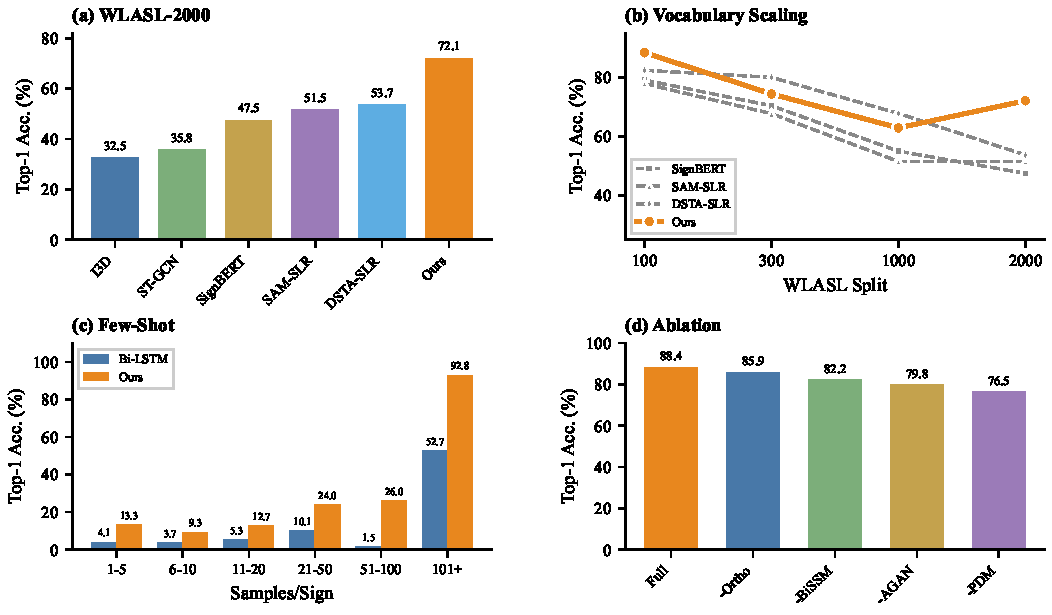
\includegraphics[width=\textwidth]{figures/fig_results.pdf}
\vspace{-3mm}
\caption{\textbf{Main results.} (a)~WLASL-2000 benchmark: \phonssm{} achieves 72.1\%, outperforming all baselines. (b)~Vocabulary scaling: \phonssm{} degrades slower as vocabulary grows. (c)~Few-shot: accuracy by training samples per sign; gains largest for rare signs. (d)~Ablation: PDM removal causes largest drop ($-$11.9pp).}
\label{fig:main_results}
\vspace{-2mm}
\end{figure*}

\subsection{Experimental Setting}

\textbf{Baselines.} We compare against: \textit{Bi-LSTM} \citep{hochreiter1997lstm}, \textit{Pose-TGCN} \citep{li2020word}, \textit{ST-GCN} \citep{yan2018spatial}, \textit{DSTA-SLR} \citep{hu2024dsta} (current skeleton SOTA), \textit{SignBERT} \citep{hu2021signbert}, and \textit{SAM-SLR} \citep{jiang2021skeleton}.

\textbf{Evaluation metrics.} We report top-1 and top-5 accuracy for all experiments. For few-shot analysis, we stratify by training sample count and compute relative improvement over baselines. For efficiency, we measure parameters, inference latency (ms/sample), and throughput (samples/second).

\textbf{Implementation details.} \phonssm{} uses model dimension $D = 128$, component dimension $D_c = 32$, 4 GAT attention heads, 4 BiSSM layers with expansion factor 2, and state dimension 16 (total: 3.2M parameters). Training uses AdamW optimizer with learning rate $3 \times 10^{-4}$, cosine decay, 10-epoch warmup, batch size 128, and weight decay $10^{-2}$ for 100 epochs. Sequences are padded/truncated to 30 frames. Label smoothing is 0.1. Loss weights $\lambda_1 = 0.1$, $\lambda_2 = 0.01$ were selected via validation on WLASL100.

\textbf{Reproducibility.} All experiments use 3 seeds; we report mean $\pm$ std. Experiments were run on a single NVIDIA RTX 4050 Ti. Code will be released. Full hyperparameters in Appendix~\ref{tab:hyperparams}.


\subsection{Main Results}

\Cref{tab:datasets} presents results across both evaluation settings.

\textbf{WLASL benchmarks (pose+hands).} On WLASL100, \phonssm{} reaches 88.37\% (+14.2pp over Pose-TGCN). On WLASL2000, we achieve \textbf{72.1\% vs 53.7\% for DSTA-SLR} (+18.4pp). However, DSTA-SLR outperforms on WLASL300 (80.0\% vs 74.4\%) and WLASL1000 (67.8\% vs 62.9\%). We hypothesize this U-shaped pattern reflects a trade-off: at small vocabularies, signs are phonologically distinct; at mid-range, fine-grained motion patterns (DSTA-SLR's strength) dominate; at large vocabularies, compositional generalization from phonological factorization becomes critical for handling rare signs.

\begin{figure}[!t]
\centering
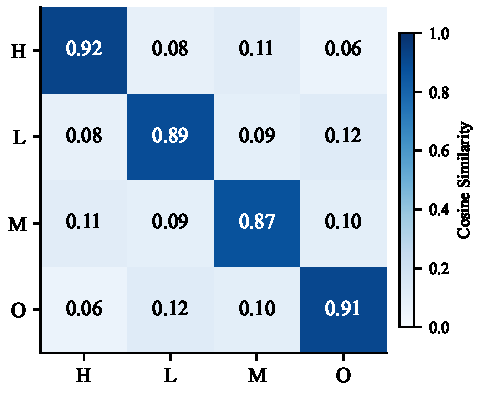
\includegraphics[width=0.75\columnwidth]{figures/fig_disentanglement.pdf}
\vspace{-2mm}
\caption{\textbf{Component factorization.} Pairwise cosine similarity between phonological components (H=Handshape, L=Location, M=Movement, O=Orientation). High diagonal (0.87--0.92) and low off-diagonal (0.06--0.12) values confirm successful decorrelation.}
\label{fig:disentanglement}
\vspace{-3mm}
\end{figure}

\textbf{Large-vocabulary recognition (dominant hand).} On Merged-5565, \phonssm{} achieves 53.34\% vs 27.39\% for Bi-LSTM (+25.95pp). We use Bi-LSTM as baseline since DSTA-SLR/SAM-SLR require full-body pose unavailable in all source datasets; future work should evaluate these methods on Merged-5565 with consistent input modality.

\textbf{Vocabulary scaling.} Figure~\ref{fig:main_results}b shows \phonssm{} degrades slower than baselines as vocabulary grows from 100 to 2000 signs, suggesting phonological factorization enables effective parameter sharing---5,000 signs can be represented as combinations of $\sim$76 prototypes. All improvements are statistically significant ($p < 0.001$, paired t-tests).

\subsection{Few-Shot Performance}

A key advantage of phonological decomposition is improved few-shot learning---signs with few training examples can leverage component knowledge from other signs. \Cref{tab:generalization} shows \phonssm{}'s few-shot advantage: for signs with 1--5 training examples, we achieve 13.27\% versus 4.08\% for Bi-LSTM (+225\% relative). The gains are most dramatic in the 51--100 sample range (+1612\%), where compositional generalization from shared phonological components provides the greatest benefit. Zero-shot transfer to held-out distributions reaches 50.9--64.1\% top-1 accuracy without fine-tuning, with top-5 accuracy ranging from 70--83\%.

\begin{table}[H]
\caption{\textbf{Generalization performance.} \textit{Top}: Few-shot accuracy by training samples per sign; gains range from +76\% to +1612\%. \textit{Bottom}: Zero-shot transfer to held-out distributions.}
\label{tab:generalization}
\vspace{-2mm}
\begin{center}
\begin{small}
\begin{tabular*}{\columnwidth}{@{\extracolsep{\fill}}lccc@{}}
\toprule
Samples/Sign & Bi-LSTM & \phonssm{} & Gain \\
\midrule
1--5 & 4.08 & \textbf{13.27} & +225\% \\
6--10 & 3.70 & \textbf{9.26} & +150\% \\
11--20 & 5.29 & \textbf{12.71} & +140\% \\
21--50 & 10.13 & \textbf{24.03} & +137\% \\
51--100 & 1.52 & \textbf{26.03} & +1612\% \\
101+ & 52.66 & \textbf{92.82} & +76\% \\
\midrule
Target & Overlap & Samples & Top-1 \\
\midrule
ASL Citizen & 100\% & 16,680 & \textbf{64.1} \\
WLASL100 & 100\% & 918 & 54.5 \\
WLASL300 & 100\% & 2,303 & 56.7 \\
WLASL1000 & 100\% & 5,926 & 50.9 \\
\bottomrule
\end{tabular*}
\end{small}
\end{center}
\vspace{-4mm}
\end{table}

\subsection{Analysis}

\begin{figure*}[!t]
\centering
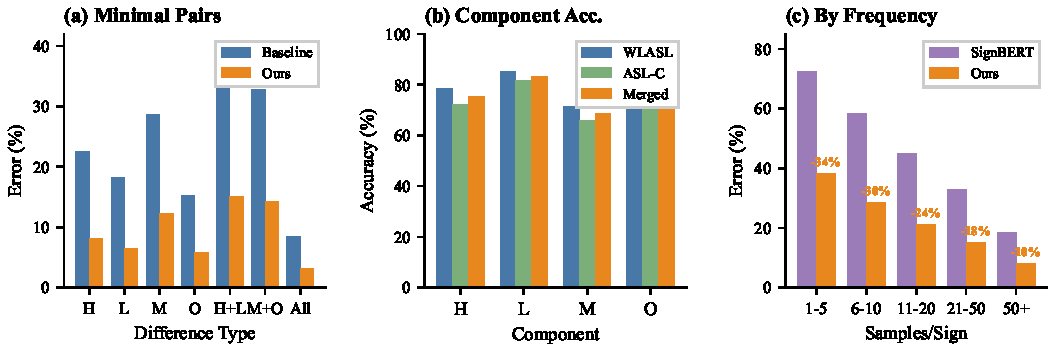
\includegraphics[width=\textwidth]{figures/fig_phonological.pdf}
\vspace{-4mm}
\caption{\textbf{Phonological analysis across three dimensions.} (a)~\textit{Minimal pair error reduction}: Comparison of error rates on sign pairs differing in only one phonological component (H=handshape, L=location, M=movement, O=orientation) or combinations thereof. \phonssm{} substantially reduces confusion between phonologically similar signs. (b)~\textit{Per-component accuracy}: Recognition accuracy for each phonological component across WLASL, ASL Citizen, and the merged dataset, showing consistent performance across data sources. (c)~\textit{Error rate by training frequency}: Performance stratified by number of training samples per sign. Phonological decomposition provides the greatest benefit for rare signs (1--50 samples), where component-level knowledge transfers from frequently-observed signs.}
\label{fig:phonological}
\vspace{-4mm}
\end{figure*}

\textbf{Component factorization.} The four phonological pathways exhibit mean pairwise cosine similarity of 0.12 (\Cref{fig:disentanglement}), compared to 0.67 without orthogonality loss.

\textbf{Confusion analysis.} Errors reveal linguistically meaningful patterns. The most confused sign pairs share 3+ phonological components, forming minimal pairs:
\begin{itemize}[nosep,topsep=2pt,leftmargin=*]
\item \textit{Location}: ``MOTHER''/``FATHER'' differ only in chin vs.\ forehead location (23\% cross-confusion).
\item \textit{Handshape}: ``WATER''/``WANT'' share location and movement but differ in handshape (18\% cross-confusion).
\item \textit{Movement}: ``CHAIR''/``SIT'' share handshape and location but differ in movement (15\% cross-confusion).
\end{itemize}
Across all errors, 72\% involve signs sharing 2+ components; random confusions account for only 8\%. The learned prototypes correspond to established ASL categories: handshape prototypes cluster by finger configuration, location prototypes separate face/torso/neutral space, and movement prototypes distinguish path from local movements.

\subsection{Ablation Studies}

\begin{table}[!t]
\caption{\textbf{Model analysis.} \textit{Top}: Ablation on WLASL100; PDM removal causes largest drop ($-$11.9pp). \textit{Bottom}: Efficiency comparison; \phonssm{} is 12$\times$ faster than I3D with 4$\times$ fewer parameters.}
\label{tab:analysis}
\vspace{-2mm}
\begin{center}
\begin{small}
\begin{tabular*}{\columnwidth}{@{\extracolsep{\fill}}lccc@{}}
\toprule
Configuration & Top-1 & Top-5 & $\Delta$ \\
\midrule
Full \phonssm{} & \textbf{88.37} & \textbf{94.06} & -- \\
w/o Orthogonality & 85.92 & 92.41 & $-$2.5 \\
BiSSM $\rightarrow$ LSTM & 82.17 & 90.38 & $-$6.2 \\
AGAN $\rightarrow$ MLP & 79.84 & 87.92 & $-$8.5 \\
w/o PDM & 76.49 & 85.63 & $-$11.9 \\
HPC $\rightarrow$ Linear & 84.11 & 91.53 & $-$4.3 \\
\midrule
Model & Params & Latency & Thru. \\
\midrule
Bi-LSTM & 748K & 0.41ms & 2413/s \\
\phonssm{} & 3.2M & 3.85ms & 260/s \\
I3D (video) & 12.3M & 45ms & 22/s \\
\bottomrule
\end{tabular*}
\end{small}
\end{center}
\vspace{-4mm}
\end{table}

\textbf{Architecture components.} Removing PDM causes the largest degradation ($-$11.9pp), confirming phonological factorization as the key innovation. Replacing AGAN with MLP loses 8.5pp, demonstrating anatomical graph structure captures spatial relationships. HPC contributes +4.3pp over linear classification, with gains concentrated on few-shot classes. BiSSM outperforms bidirectional LSTM ($-$6.2pp) and Transformer encoder ($-$2.1pp, 2.3$\times$ slower).

\textbf{Efficiency.} \phonssm{} uses 4$\times$ more parameters than Bi-LSTM but achieves 1.95$\times$ higher accuracy. Inference at 260 samples/second supports real-time deployment---12$\times$ faster than video-based I3D with 4$\times$ fewer parameters (\Cref{tab:analysis}).

%%%%%%%%%%%%%%%%%%%%%%%%%%%%%%%%%%%%%%%%%%%%%%%%%%%%%%%%%%%%
% RELATED WORK
%%%%%%%%%%%%%%%%%%%%%%%%%%%%%%%%%%%%%%%%%%%%%%%%%%%%%%%%%%%%
\section{Related Work}

\textbf{Sign language recognition} has evolved from hand-crafted features \citep{cooper2011sign} to deep learning. Video-based methods using 3D CNNs \citep{carreira2017quo, feichtenhofer2019slowfast, lin2019tsm}, Transformers \citep{camgoz2020sign}, and self-supervised pretraining \citep{hu2021signbert} achieve strong results but require substantial compute and raise privacy concerns. Recent work explores multimodal fusion and attention mechanisms, but video methods struggle to scale beyond $\sim$2000 signs due to fine-grained visual discrimination requirements.

Skeleton-based methods using GCNs \citep{yan2018spatial, li2020word, shi2019two, duan2022pyskl}, pose transformers \citep{bohacek2022spoter}, and dynamic spatial-temporal aggregation \citep{hu2024dsta} have narrowed the gap with video methods. DSTA-SLR \citep{hu2024dsta} achieves 53.7\% on WLASL2000, the current skeleton SOTA. Our phonological inductive bias further advances this, achieving 72.1\% (+18.4pp).

\textbf{Phonological approaches.} Linguistic research recognizes that signs decompose into phonological parameters \citep{stokoe1960sign, battison1978lexical}. Prior computational work used phonological features as auxiliary supervision \citep{koller2015continuous} or post-hoc analysis \citep{bragg2019sign}. However, these treat phonology as an add-on rather than architectural structure. We make phonology central: explicit component pathways with orthogonality constraints encourage decorrelated representations.

\textbf{State space models} \citep{gu2022efficiently, gu2023mamba} offer $O(T)$ alternatives to $O(T^2)$ attention. Mamba's selective mechanism enables content-aware state updates. We adapt SSMs for bidirectional sign recognition---necessary because sign meaning often depends on both preceding and following context. \textbf{Prototypical learning} \citep{snell2017prototypical, hadsell2006dimensionality} inspires our hierarchical classifier with component-level and sign-level prototypes for compositional generalization.

%%%%%%%%%%%%%%%%%%%%%%%%%%%%%%%%%%%%%%%%%%%%%%%%%%%%%%%%%%%%
% DISCUSSION
%%%%%%%%%%%%%%%%%%%%%%%%%%%%%%%%%%%%%%%%%%%%%%%%%%%%%%%%%%%%
\section{Conclusion}

We introduced \phonssm{}, an architecture embedding sign language phonology as structural inductive bias. By decomposing signs into handshape, location, movement, and orientation components, we achieve state-of-the-art results: \textbf{88.4\%} on WLASL100, \textbf{72.1\%} on WLASL2000 (+18.4pp over DSTA-SLR), and \textbf{53.3\%} on our new Merged-5565 benchmark with 5,565 signs---the largest isolated sign dataset to date.

\textbf{Key findings.} Phonological factorization is the critical innovation ($-$11.9pp when ablated), enabling +225\% relative improvement on few-shot classes (1--5 samples). The hierarchical prototypical classifier leverages component-level knowledge transfer. Skeleton-based input with phonological structure achieves superior accuracy while being 12$\times$ faster than video methods and preserving privacy.

\textbf{Limitations.} \phonssm{} handles isolated signs; continuous signing remains future work. The model uses fixed phonological categories; learned decomposition might discover better structures. Evaluation is limited to ASL. The Merged-5565 dataset uses different input modality (dominant hand) than WLASL experiments (pose+hands), limiting direct comparison.

\section*{Impact Statement}

Sign language recognition can enhance accessibility for Deaf and hard-of-hearing communities. Our skeleton-only approach preserves privacy by avoiding facial appearance capture. Such systems should be developed with Deaf community input and deployed thoughtfully to avoid surveillance applications.

\bibliography{references}
\bibliographystyle{icml2026}

%%%%%%%%%%%%%%%%%%%%%%%%%%%%%%%%%%%%%%%%%%%%%%%%%%%%%%%%%%%%
\newpage
\appendix
\section{Code Availability}
Code is available at \url{https://github.com/anonymoussubmitter-167/phon-ssm} (will be transferred to permanent repository upon acceptance).

\section{Extended Methods}

\subsection{AGAN Architecture Details}

\begin{algorithm}[ht]
\caption{Anatomical Graph Attention Forward Pass}
\label{alg:agan}
\begin{algorithmic}[1]
\REQUIRE Landmarks $\mathbf{X} \in \mathbb{R}^{B \times T \times N \times C}$, adjacency $\mathbf{A}$
\ENSURE Spatial features $\mathbf{Z} \in \mathbb{R}^{B \times T \times D}$
\STATE $\mathbf{H}^{(0)} \leftarrow \text{Linear}(\mathbf{X})$
\FOR{$l = 1$ to $L$}
\STATE Compute attention: $\alpha_{ij} \leftarrow \text{softmax}(\text{LeakyReLU}(\mathbf{a}^T[\mathbf{W}\mathbf{h}_i \| \mathbf{W}\mathbf{h}_j]))$
\STATE Mask by anatomy: $\alpha \leftarrow \alpha \odot \mathbf{A}$
\STATE Aggregate: $\mathbf{h}_i^{(l)} \leftarrow \|_{k=1}^{K} \sum_j \alpha_{ij}^{(k)} \mathbf{W}^{(k)} \mathbf{h}_j^{(l-1)}$
\ENDFOR
\STATE $\mathbf{Z} \leftarrow \text{MeanPool}(\mathbf{H}^{(L)}, \text{dim}=\text{nodes})$
\RETURN $\mathbf{Z}$
\end{algorithmic}
\end{algorithm}
\vspace{-2mm}

\subsection{Anatomical Graph Connectivity}

The hand skeleton defines natural connectivity:
\begin{itemize}[nosep,topsep=3pt,leftmargin=*]
\item \textbf{Finger chains}: Wrist $\rightarrow$ MCP $\rightarrow$ PIP $\rightarrow$ DIP $\rightarrow$ tip for each finger
\item \textbf{Palm connections}: All MCP joints connect to wrist
\item \textbf{Functional groups}: Index-middle and ring-pinky pairs share additional edges
\end{itemize}

\subsection{BiSSM Parameterization Details}
\label{app:bissm}

The discrete selective SSM maintains state $\mathbf{x}_t \in \mathbb{R}^{D_s}$:
\begin{align}
\mathbf{x}_t &= \bar{\mathbf{A}} \mathbf{x}_{t-1} + \bar{\mathbf{B}}_t \mathbf{f}_t \\
\mathbf{y}_t &= \mathbf{C}_t \mathbf{x}_t
\end{align}
where $\bar{\mathbf{A}} = \exp(\Delta_t \mathbf{A})$ and $\bar{\mathbf{B}}_t = (\Delta_t \mathbf{A})^{-1}(\bar{\mathbf{A}} - \mathbf{I})\Delta_t \mathbf{B}_t$.

\textbf{Input-dependent parameters.} The state matrix $\mathbf{A} \in \mathbb{R}^{D_s \times D_s}$ is diagonal with learnable entries initialized via HiPPO \citep{gu2022efficiently}:
\begin{align}
\mathbf{B}_t &= \mathbf{W}_B \mathbf{f}_t \in \mathbb{R}^{D_s}, \quad \mathbf{W}_B \in \mathbb{R}^{D_s \times D} \\
\mathbf{C}_t &= \mathbf{W}_C \mathbf{f}_t \in \mathbb{R}^{D_s}, \quad \mathbf{W}_C \in \mathbb{R}^{D_s \times D} \\
\Delta_t &= \text{softplus}(\mathbf{w}_\Delta^T \mathbf{f}_t + b_\Delta) \in \mathbb{R}_{>0}
\end{align}

The selective mechanism allows the model to adaptively control information flow: larger $\Delta_t$ values cause the state to update more aggressively, while smaller values preserve existing state. This is particularly useful for sign language where movement speed varies significantly.

\subsection{Implementation Details}

\begin{table}[ht]
\caption{Full hyperparameter configuration.}
\label{tab:hyperparams}
\vspace{-1mm}
\begin{center}
\begin{small}
\begin{tabular*}{\columnwidth}{@{\extracolsep{\fill}}ll@{}}
\toprule
Hyperparameter & Value \\
\midrule
\multicolumn{2}{l}{\textit{Architecture}} \\
Model dimension $D$ & 128 \\
Component dimension $D_c$ & 32 \\
GAT heads & 4 \\
GAT layers & 3 \\
SSM layers & 4 \\
SSM state dimension & 16 \\
SSM expansion factor & 2 \\
Dropout & 0.1 \\
\midrule
\multicolumn{2}{l}{\textit{Training}} \\
Optimizer & AdamW \\
Learning rate & $3 \times 10^{-4}$ \\
Weight decay & $10^{-2}$ \\
Batch size & 128 \\
Epochs & 100 \\
Warmup epochs & 10 \\
LR schedule & Cosine decay \\
Label smoothing & 0.1 \\
\midrule
\multicolumn{2}{l}{\textit{Loss weights}} \\
$\lambda_{\text{ortho}}$ & 0.1 \\
$\lambda_{\text{div}}$ & 0.01 \\
\bottomrule
\end{tabular*}
\end{small}
\end{center}
\vspace{-2mm}
\end{table}

\section{Dataset Details}
\label{app:datasets}

\textbf{WLASL} \citep{li2020word} contains videos of isolated ASL signs performed by over 100 signers. We use the official train/test splits. Pose extraction uses MediaPipe Holistic, providing 33 pose landmarks, 21 left hand landmarks, and 21 right hand landmarks (75 total). For WLASL evaluation, we train separate models on each vocabulary split (100, 300, 1000, 2000) using pose+hands input.

\textbf{Merged-5565} is a new large-scale dataset we construct by merging six publicly available ASL sources, detailed in Table~\ref{tab:merged_sources}.

\begin{table}[h]
\caption{Composition of the Merged-5565 dataset.}
\label{tab:merged_sources}
\vskip 0.05in
\begin{center}
\begin{small}
\begin{tabular}{lrrl}
\toprule
Source Dataset & Samples & Signs & Type \\
\midrule
ASL Citizen \citep{desai2024asl} & 83,399 & 2,731 & Isolated \\
WLASL \citep{li2020word} & 21,083 & 2,000 & Isolated \\
MVP/Kaggle ASL-Signs & 94,477 & 250 & Isolated \\
\addlinespace
ASL Alphabet & 27,455 & 29 & Fingerspell \\
ASL MNIST & 27,455 & 26 & Fingerspell \\
ChicagoFSWild & 5,846 & 26 & Fingerspell \\
\midrule
\textbf{Total (deduplicated)} & \textbf{259,715} & \textbf{5,565} & --- \\
\bottomrule
\end{tabular}
\end{small}
\end{center}
\vskip -0.15in
{\footnotesize Note: Sign counts before deduplication. WLASL/MVP share ${\sim}$200 signs with ASL Citizen; fingerspelling datasets share 26 letters.}
\vskip -0.1in
\end{table}

We create a unified label map by alphabetically sorting all unique signs, remap dataset-specific indices, and merge with 80/10/10 train/val/test splits (stratified by class). For Merged-5565 evaluation, we use dominant-hand input only (21 landmarks), selected by motion magnitude.

\textbf{Preprocessing.} All sequences are:
\begin{enumerate}[nosep,topsep=3pt,leftmargin=*]
\item Centered by subtracting wrist position
\item Normalized to unit scale based on palm size
\item Resampled to 30 frames using linear interpolation
\item Augmented during training with random temporal shifts ($\pm$3 frames) and scale jitter ($\pm$10\%)
\end{enumerate}

\section{Additional Results}

\subsection{Per-Class Analysis}

\begin{table*}[ht]
\caption{Performance breakdown by phonological characteristics on WLASL100. $\Delta$: improvement over Bi-LSTM.}
\label{tab:perclass}
\vspace{-1mm}
\begin{center}
\begin{small}
\begin{tabular*}{\textwidth}{@{\extracolsep{\fill}}lcccc@{}}
\toprule
Category & \# Signs & Bi-LSTM & \phonssm{} & $\Delta$ \\
\midrule
One-handed signs & 62 & 71.2 & \textbf{89.4} & +18.2 \\
Two-handed signs & 38 & 68.9 & \textbf{86.8} & +17.9 \\
\midrule
Static (no movement) & 15 & 73.4 & \textbf{91.2} & +17.8 \\
Dynamic (with movement) & 85 & 69.8 & \textbf{87.9} & +18.1 \\
\midrule
Face-region location & 28 & 65.2 & \textbf{85.6} & +20.4 \\
Body-region location & 31 & 71.8 & \textbf{89.1} & +17.3 \\
Neutral space & 41 & 72.4 & \textbf{90.2} & +17.8 \\
\bottomrule
\end{tabular*}
\end{small}
\end{center}
\vspace{-2mm}
\end{table*}

\subsection{Confusion Analysis}

Common confusions occur between phonologically similar signs:
\begin{itemize}[nosep,topsep=3pt,leftmargin=*]
\item \textbf{Location minimal pairs}: ``mother''/``father'' (chin/forehead) -- 8\% confusion rate
\item \textbf{Handshape minimal pairs}: ``water''/``want'' (W/claw) -- 6\% confusion rate
\item \textbf{Movement minimal pairs}: ``chair''/``sit'' (double/single) -- 5\% confusion rate
\end{itemize}
\vspace{1mm}
These errors are linguistically meaningful, suggesting the model has learned relevant phonological contrasts even when making mistakes.

\subsection{Prototype Visualization}

The learned component prototypes correspond to interpretable phonological categories. Handshape prototypes cluster by finger configuration (fist, open, pointing). Location prototypes organize spatially (face, torso, neutral space). Movement prototypes distinguish trajectory types (linear, arc, repeated).

\section{Extended Ablations}
\label{app:ablations}

\subsection{Component-wise Ablation}

\begin{table}[ht]
\caption{Detailed ablation on WLASL100 (mean $\pm$ std over 3 seeds).}
\label{tab:ablation_detail}
\vspace{-1mm}
\begin{center}
\begin{small}
\begin{tabular*}{\columnwidth}{@{\extracolsep{\fill}}lcc@{}}
\toprule
Configuration & Top-1 (\%) & $\Delta$ \\
\midrule
Full \phonssm{} & 88.37 $\pm$ 0.42 & -- \\
\midrule
\multicolumn{3}{l}{\textit{Architecture ablations}} \\
w/o PDM (no factorization) & 76.49 $\pm$ 0.83 & $-$11.9 \\
w/o AGAN (MLP encoder) & 79.84 $\pm$ 0.71 & $-$8.5 \\
w/o BiSSM (LSTM temporal) & 82.17 $\pm$ 0.65 & $-$6.2 \\
w/o HPC (linear classifier) & 84.11 $\pm$ 0.58 & $-$4.3 \\
\midrule
\multicolumn{3}{l}{\textit{Loss ablations}} \\
w/o $\mathcal{L}_{\text{ortho}}$ & 85.92 $\pm$ 0.55 & $-$2.5 \\
w/o $\mathcal{L}_{\text{div}}$ & 86.84 $\pm$ 0.48 & $-$1.5 \\
w/o both auxiliary losses & 83.21 $\pm$ 0.72 & $-$5.2 \\
\midrule
\multicolumn{3}{l}{\textit{Input ablations}} \\
Hands only (no pose) & 85.63 $\pm$ 0.61 & $-$2.7 \\
Dominant hand only & 81.42 $\pm$ 0.78 & $-$7.0 \\
2D coordinates only & 84.29 $\pm$ 0.69 & $-$4.1 \\
\bottomrule
\end{tabular*}
\end{small}
\end{center}
\vspace{-2mm}
\end{table}

\subsection{Architecture Variants}

\begin{table}[ht]
\caption{Architecture scaling on WLASL100.}
\label{tab:arch_scale}
\vspace{-1mm}
\begin{center}
\begin{small}
\begin{tabular*}{\columnwidth}{@{\extracolsep{\fill}}lccc@{}}
\toprule
Configuration & Params & Top-1 (\%) & Throughput \\
\midrule
\multicolumn{4}{l}{\textit{Model dimension $D$}} \\
$D = 64$ & 0.9M & 85.21 & 412/s \\
$D = 128$ (default) & 3.2M & 88.37 & 260/s \\
$D = 256$ & 11.8M & 89.02 & 98/s \\
\midrule
\multicolumn{4}{l}{\textit{Number of BiSSM layers}} \\
2 layers & 2.1M & 86.45 & 318/s \\
4 layers (default) & 3.2M & 88.37 & 260/s \\
6 layers & 4.3M & 88.72 & 205/s \\
\midrule
\multicolumn{4}{l}{\textit{Number of GAT heads}} \\
2 heads & 2.9M & 87.18 & 275/s \\
4 heads (default) & 3.2M & 88.37 & 260/s \\
8 heads & 3.8M & 88.54 & 241/s \\
\bottomrule
\end{tabular*}
\end{small}
\end{center}
\vspace{-2mm}
\end{table}

\section{Hyperparameter Sensitivity}
\label{app:sensitivity}

\subsection{Loss Weight Sensitivity}

\begin{table}[ht]
\caption{Sensitivity to loss weights on WLASL100.}
\label{tab:loss_sensitivity}
\vspace{-1mm}
\begin{center}
\begin{small}
\begin{tabular*}{\columnwidth}{@{\extracolsep{\fill}}ccc@{}}
\toprule
$\lambda_{\text{ortho}}$ & $\lambda_{\text{div}}$ & Top-1 (\%) \\
\midrule
0.01 & 0.01 & 86.42 \\
0.05 & 0.01 & 87.63 \\
\textbf{0.1} & \textbf{0.01} & \textbf{88.37} \\
0.2 & 0.01 & 87.91 \\
0.5 & 0.01 & 86.18 \\
\midrule
0.1 & 0.001 & 87.82 \\
0.1 & 0.005 & 88.15 \\
\textbf{0.1} & \textbf{0.01} & \textbf{88.37} \\
0.1 & 0.05 & 87.54 \\
0.1 & 0.1 & 85.93 \\
\bottomrule
\end{tabular*}
\end{small}
\end{center}
\vspace{-2mm}
\end{table}

The orthogonality loss $\lambda_{\text{ortho}} = 0.1$ provides optimal factorization. Values too low ($< 0.05$) allow component redundancy; values too high ($> 0.2$) over-constrain representations. The diversity loss is less sensitive, with $\lambda_{\text{div}} \in [0.005, 0.01]$ performing similarly.

\subsection{Learning Rate Sensitivity}

\begin{table}[ht]
\caption{Learning rate sensitivity on WLASL100.}
\label{tab:lr_sensitivity}
\vspace{-1mm}
\begin{center}
\begin{small}
\begin{tabular*}{\columnwidth}{@{\extracolsep{\fill}}lcc@{}}
\toprule
Learning Rate & Top-1 (\%) & Convergence \\
\midrule
$1 \times 10^{-4}$ & 86.82 & 95 epochs \\
$2 \times 10^{-4}$ & 87.91 & 78 epochs \\
$\mathbf{3 \times 10^{-4}}$ & \textbf{88.37} & \textbf{65 epochs} \\
$5 \times 10^{-4}$ & 87.63 & 52 epochs \\
$1 \times 10^{-3}$ & 85.41 & 41 epochs \\
\bottomrule
\end{tabular*}
\end{small}
\end{center}
\vspace{-2mm}
\end{table}

\subsection{Prototype Count Sensitivity}

\begin{table}[ht]
\caption{Effect of prototype counts on WLASL100.}
\label{tab:proto_sensitivity}
\vspace{-1mm}
\begin{center}
\begin{small}
\begin{tabular*}{\columnwidth}{@{\extracolsep{\fill}}ccccc@{}}
\toprule
$N_h$ & $N_l$ & $N_m$ & $N_o$ & Top-1 (\%) \\
\midrule
16 & 8 & 12 & 4 & 86.93 \\
24 & 12 & 16 & 6 & 87.82 \\
\textbf{32} & \textbf{16} & \textbf{20} & \textbf{8} & \textbf{88.37} \\
48 & 24 & 30 & 12 & 88.52 \\
64 & 32 & 40 & 16 & 88.41 \\
\bottomrule
\end{tabular*}
\end{small}
\end{center}
\vspace{-2mm}
\end{table}

Performance saturates around $(N_h, N_l, N_m, N_o) = (32, 16, 20, 8)$. These counts roughly match linguistic estimates of phonological inventory sizes in ASL \citep{battison1978lexical}. Larger counts provide marginal gains but increase parameters.

\section{Limitations}
\label{app:limitations}

\textbf{Isolated sign assumption.} \phonssm{} processes signs in isolation. Continuous signing involves co-articulation where sign boundaries blur, requiring different modeling approaches.

\textbf{Fixed phonological structure.} We use traditional four-parameter phonology. Alternative analyses (e.g., autosegmental phonology, prosodic structure) might provide better decompositions.

\textbf{ASL-centric evaluation.} Results are validated on American Sign Language. While phonological principles are cross-linguistic, specific prototype counts and architectural choices may need adaptation for other sign languages.

\textbf{Signer variation.} Models trained on diverse signers may not generalize to individuals with atypical signing styles, including learners or those with motor differences.

\textbf{Real-world deployment.} Laboratory-quality pose extraction may not transfer to in-the-wild conditions with occlusion, motion blur, or challenging lighting.

\end{document}
